\chapter{\xlabel{pol2_dr}POL-2 Data Reduction - The Theory}
\label{sec:dr}
\section{\xlabel{dataflow}The Data Flow}

POL-2 data reduction is a complex and involved process for which a broad overview is presented first before
the specific details are discussed. It is noted that this same procedure is used whether there is one or 
multiple observation to reduce.

The data reduction process can be broken down into three main steps as shown in Figure \ref{fig:pol2drflow}.

\begin{figure}[t!]
\begin{center}
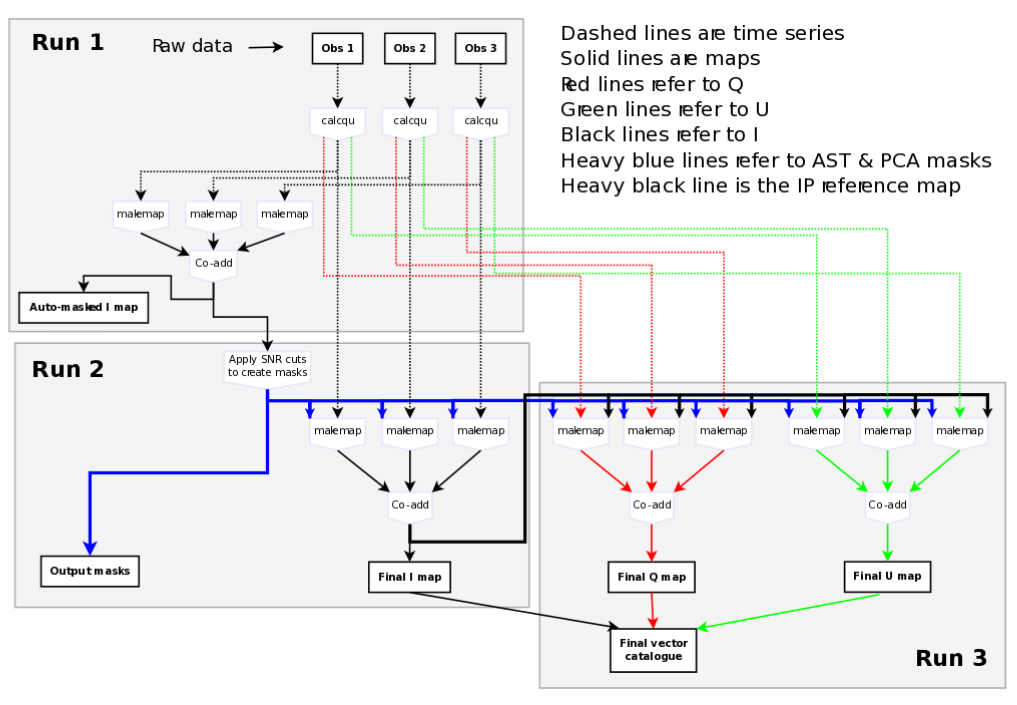
\includegraphics[width=0.95\linewidth]{pol2-dr-flow.png}
\label{fig:pol2drflow}
\caption [POL-2 Data Flow]{
  \small The data flow of the POL-2 data reduction method is
  presented. In this example three POL-2 observations are
  reduced and combined in various stages and combination to
  produce I, Q and U maps.
}
\end{center}
\end{figure}


\subsection*{Step 1}

The initial step of the process (see Run 1 in Figure \cite{fig:pol2drflow}) creates 
an intensity, I, map from the raw data files provided to the reduction routine (see \cref{Chapter}{sec:rundr}). 


\subsubsection*{The process}
The  analysed  intensity values in the raw data time-streams are first converted into Q, U and I time-streams
using smurf:calcqu (these are stored for future use in the directory qudata, specified by the qudir parameter in the example command below). 

The smurf:makemap command is then used to create a separate map from the I time-stream for each observation, using SNR-based “auto-masking” to define the background regions that are to be set to zero at the end of each iteration.  

These maps are stored for future use in the directory maps, specified by the mapdir parameter. Each map has a name of the form:

<UT_DATE>_<OBS_NUM>_<CHUNK_NUM>_imap.sdf

where <CHUNK_NUM> indicates the raw data file at the start of the contiguous chunk of data used to create the map, and is
usually 0003. Each of these maps is compared to the specified reference map (if any) to determine a pointing correction to be applied to the observation in future
2 . If no reference map is supplied, the I map created from the first observation defines the expected source position, and is compared with later maps to determine their pointing corrections.


\subsection*{Step 2}

In the second step of the process (see Run 2 in Figure \ref{fig:pol2drflow}) an improved I map is produced. This improvements come from i) applied relative pointing corrections 


\subsection*{Step 3}

In the third step of the reduction process (see Run 3 in Figure \ref{fig:pol2drflow}) both the Q and U maps are produced. The production of the Q and U maps requires the raw Q and U data, the final I map (produced in step 2) and the output masks (also produced in step 2). Once the Q and U maps are produced a final vector catalogue is created.

\section{\xlabel{makemap}Makemap}

The POL-2 data reduction builds upon the SCUBA-2 make-map data reduction. The Dynamic Iterative Map-Maker, hereafter just referred to as the map-maker is the tool you will use to produce SCUBA-2 maps, and is implemented by the Smurf makemap command. It performs all pre-processing steps to clean the data, followed by solving for multiple signal components using an iterative algorithm, and binning the resulting time-series data to produce a final science map. 




\section{\xlabel{pca}PCA}

One difference in the reduction of SCUBA-2 data and POL-2 data is the method for sky removal. 
In the case of POl-2 this must also include the polarized sky background. 
For those familiar with SCUBA-2 reductions this is done using the COM/GAI model. 

The COM/GAI model assumes the background is common to all bolometers (after gain variations between bolometers). This would be the case if both the sky brightness and the instrumental polarization was constant across the focal plane. 

In pol2map, the reduction command for POL-2 data, the sky removal is done using PCA, Principle Component Analysis.
The PCA approach allows there to be multiple correlated components with different amplitudes at different points in the focal plane.


It \emph{is} possible to run PCA on SCUBA-2 data but the return is minimal. 



\section{\xlabel{masking}Masking}
A mask is a two-dimensional array which has the same shape and size as the final map, and
which is used to indicate where the source is expected to fall within the map. Bad pixel values
within a mask indicate background pixels, and good pixels values indicate source pixels. Masks
are used for two main purposes:

\begin{enumerate}\itemsep-0.2em
\item To prevent the growth of gradients and other artificial large scale structures within the
map.  For this purpose, the astronomical signal at all background pixels defined by the
mask is forced to zero at the end of each iteration within makemap (except for the final iteration).
\item To prevent bright sources polluting the evaluation of the various noise models (PCA, COM, FLT) used within
makemap. Source pixels are excluded from the calculation of these models.
\end{enumerate}


The pol2map script uses different masks for these two purposes - the “AST” mask and the “PCA” mask. 
The PCA mask is in general less extensive than the AST mask, with the source areas being restricted to the brighter inner regions.
Each of these two masks can either be generated automatically within makemap, or be specified by
a fixed external NDF. 


\section{\xlabel{config}The pol2 dimmconfig file}
\label{sec:config}



not to be directly used (hence hidden) .dimmconfig\_pol2.lis
numiter = -5




\begin{terminalv}
#  Use PCA to model and remove the  background polarisation.
   modelorder = (pca,ext,ast,noi)

#  Time based despiking.
   spikebox = 10
   spikethresh = 5

#  POL" scans are very slow, so avoid flagging slow samples.
   flagslow = 0.01

#  Aggreive noise clipping.
   noisecliphigh = 3

#  The data has already been downsampled by CALCQU, so don't  do any more
#  down sampling.
   downsampscale = 0

#  Weight bolometers using the RMS residuals calculated by CALQU and
#  stored i nthe variance component of the CALCQU output NDFs.
   noi.usevar = 1

#  Use smaller boxes when finding DC steps because of the very low sample
#  rate of POL2 Stokes vector time-series created by calcqu.
   dcfitbox = 5
   dcsmooth = 10
\end{terminalv}


\subsection{dimmconfig\_pol2\_compact.lis}

This reduction builds on the default dimmconfig\_pol2.lis configuration file but uses boundary 
constraints for an initial ast mask since the source is assumed to be isolated.


\begin{terminalv}
   ast.zero_circle = (0.016666)
\end{terminalv}


\subsection{dimmconfig\_pol2\_extended.lis}


This reduction builds on the default dimmconfig\_pol2.lis configuration file but

\begin{terminalv}
   numiter=-40
   ast.zero_snr = 3
   ast.zero_snrlo = 2
\end{terminalv}


\section{\xlabel{addingdata}Adding new observations}



\section{\xlabel{tailoredDR}Tailoring your reduction}

\subsection*{variances between POL-2 maps}

MAPVAR is a parameter that controls the variances in the coadded 
I, Q and U maps are formed.

If  MAPVAR is set TRUE, the variances in the coadded I, Q and U maps
are formed from the spread of pixel data values in the individual
observation maps. If MAPVAR is FALSE (the default), the variances in
the coadded maps are formed (as in previous versions of pol2map) by
propagating the pixel variance values created by makemap from the
individual observation maps.

Only use MAPVAR=TRUE if you have enough observations to
make the variances between them meaningful. It's hard to put a lower
limit on it, but it is advised that at a minimum 10 observations.


If you want to test the effect of this option on a field for which you
already have the I, Q and U maps from a set of individual
observations, you can do the following:

\begin{terminalv}
% pol2map in=maps/\* iout=imapvar qout=qmapvar uout=umapvar mapvar=yes \
                   ipcor=no cat=cat_mapvar debias=yes
\end{terminalv}

assuming your I, Q and U maps are in directory "maps". The variances
in imapvar.sdf qmapvar.sdf and umapvar.sdf will be calculated using
the new method, and these variances will then be used to form the
errors in the cat_mapvar.FIT catalogue.



